% ============================================================
%  keyMappings.tex
%  Key Findings — Geometry of the Virtue of Complexity
%  Fully self-contained: compile with pdflatex (twice for refs)
%    pdflatex keyMappings.tex
% ============================================================
\documentclass[11pt,a4paper]{article}

% ── Packages ─────────────────────────────────────────────────
\usepackage[a4paper, margin=22mm]{geometry}
\usepackage{pgfplots}
\pgfplotsset{compat=1.18}
\usepackage{pgfplotstable}
\usepackage{tikz}
\usetikzlibrary{matrix, positioning}
\usepackage{booktabs}
\usepackage{array}
\usepackage{colortbl}
\usepackage{xcolor}
\usepackage{amsmath, amssymb}
\usepackage{mathtools}
\usepackage[protrusion=true,expansion=false,nopatch=eqnum]{microtype}
\usepackage{parskip}
\usepackage{hyperref}
\usepackage{caption}
\usepackage{subcaption}
\usepackage{mdframed}
\usepackage{enumitem}
\usepackage{multirow}
\usepackage[T1]{fontenc}


% ── Colours ──────────────────────────────────────────────────
\definecolor{cblue}{HTML}{185FA5}
\definecolor{ccoral}{HTML}{D85A30}
\definecolor{cgray}{HTML}{888780}
\definecolor{camber}{HTML}{BA7517}
\definecolor{cgreen}{HTML}{3B6D11}
\definecolor{cpurple}{HTML}{534AB7}
\definecolor{cred}{HTML}{A32D2D}
\definecolor{lightblue}{HTML}{E6F1FB}
\definecolor{lightgreen}{HTML}{E1F5EE}
\definecolor{lightred}{HTML}{FCEBEB}
\definecolor{rowalt}{HTML}{F1EFE8}
\definecolor{headbg}{HTML}{2C2C2A}
\definecolor{headfg}{HTML}{F1EFE8}

% ── Formula box ──────────────────────────────────────────────
\newmdenv[
  backgroundcolor=lightblue,
  linecolor=cblue,
  linewidth=0.5pt,
  innerleftmargin=8pt,
  innerrightmargin=8pt,
  innertopmargin=5pt,
  innerbottommargin=5pt,
  skipabove=4pt,
  skipbelow=4pt
]{formulabox}

\newmdenv[
  backgroundcolor=lightgreen,
  linecolor=cgreen,
  linewidth=1.5pt,
  leftline=true, rightline=false, topline=false, bottomline=false,
  innerleftmargin=8pt,
  innerrightmargin=8pt,
  innertopmargin=5pt,
  innerbottommargin=5pt,
  skipabove=4pt,
  skipbelow=4pt
]{anngreen}

\newmdenv[
  backgroundcolor=lightblue,
  linecolor=cblue,
  linewidth=1.5pt,
  leftline=true, rightline=false, topline=false, bottomline=false,
  innerleftmargin=8pt,
  innerrightmargin=8pt,
  innertopmargin=5pt,
  innerbottommargin=5pt,
  skipabove=4pt,
  skipbelow=4pt
]{annblue}

\newmdenv[
  backgroundcolor=lightred,
  linecolor=cred,
  linewidth=1.5pt,
  leftline=true, rightline=false, topline=false, bottomline=false,
  innerleftmargin=8pt,
  innerrightmargin=8pt,
  innertopmargin=5pt,
  innerbottommargin=5pt,
  skipabove=4pt,
  skipbelow=4pt
]{annred}

% ── PGFPlots defaults ─────────────────────────────────────────
\pgfplotsset{
  every axis/.style={
    axis lines=left,
    tick style={thin, color=black!40},
    grid=major,
    grid style={dotted, color=black!15},
    label style={font=\small},
    tick label style={font=\footnotesize},
    legend style={font=\footnotesize, draw=none, fill=none},
    width=0.46\textwidth,
    height=6cm,
  }
}

% ── Misc ─────────────────────────────────────────────────────
\captionsetup{font=small, labelfont=bf, skip=4pt}
\setlist[itemize]{noitemsep, topsep=2pt}

% ─────────────────────────────────────────────────────────────
\begin{document}
% ─────────────────────────────────────────────────────────────

\begin{center}
  {\LARGE\bfseries Key Findings: Geometry of the Virtue of Complexity}\\[6pt]
  {\normalsize 5-year rolling backtest $\;\cdot\;$ 35 stocks $\;\cdot\;$ 6 simulation runs
  $\;\cdot\;$ mapped to the Geometry of Complexity paper}
\end{center}
\noindent\rule{\textwidth}{0.4pt}

% ═══════════════════════════════════════════════════════════
\section*{Background}

The IPCA model relates returns $r_t \in \mathbb{R}^N$ to characteristics through
\[
  r_t \;=\; Z_t\,\Gamma^\top f_t + \varepsilon_t,
  \qquad \Gamma \in \mathrm{Mat}_{k,m}(\mathbb{R}),\quad f_t \in \mathbb{R}^k.
\]
$\Gamma$ is identified only through its row space
$W = \mathrm{row}(\Gamma) = \mathrm{span}(\Gamma^\top) \in \mathrm{Gr}(k,m)$.
After profiling out factors, the objective is a projection functional over the Grassmannian:
\[
  L(W) \;=\; \frac{1}{T}\sum_{t=1}^T \bigl\|\bigl(I - \Pi_{V_t}\bigr)r_t\bigr\|^2,
  \qquad V_t = \mathrm{span}(Z_t\Gamma^\top) \in \mathrm{Gr}(k,N).
\]
With RFF lifting, $Z_t$ is mapped to $\Phi(Z_t)\in\mathbb{R}^{N\times P}$, expanding
the admissible subspace family without changing rank $k$.
The estimator uses Riemannian conjugate gradient on $\mathrm{Gr}(m,k)$ with warm-starting.

% ═══════════════════════════════════════════════════════════
\section*{Diagnostic metrics}

All metrics are computed from the fitted $W_t \in \mathrm{Gr}(k,m)$ and the
in-window factor series $\hat{f}$.

\medskip
\textbf{Sharpe ratio} \hfill{\small Performance anchor — Section 7 criterion (iv)}
\begin{formulabox}
$\mathrm{SR} = \dfrac{\mathrm{mean}(r_{\mathrm{port},t})}{\mathrm{std}(r_{\mathrm{port},t})}
\times \sqrt{12}, \quad
r_{\mathrm{port},t} = \tfrac{1}{N}\sum_i \mathrm{pos}_{i,t}\,r_{i,t},\quad
\mathrm{pos}_{i,t} = \hat{r}_{i,t}\,/\,\tfrac{1}{N}\sum_i|\hat{r}_{i,t}|$
\end{formulabox}
{\small\color{cgray} $r_t\in\mathbb{R}^N$: cross-sectional returns (paper Eq.~1).
$\hat{r}_{i,t} = \Pi_{V_t}r_t$: projected return prediction.}

\medskip
\textbf{Subspace stability $d_{\mathrm{proj}}$} \hfill{\small Section 4.2, Eq.~17--18}
\begin{formulabox}
$d_{\mathrm{proj}}(t) = \|\Pi_{V_t} - \Pi_{V_{t-1}}\|_F
= \sqrt{2\sum_{i=1}^k \sin^2\theta_i},
\quad \max = \sqrt{2k}$
\end{formulabox}
{\small\color{cgray}
$\Pi_{V_t}=W_tW_t^\top$: projector onto $V_t\in\mathrm{Gr}(k,m)$.
$\theta_i = \arccos\sigma_i(W_t^\top W_{t-1})$: $k$ principal angles.
\emph{Note: currently confounded by random restarts — see Finding~4.}}

\medskip
\textbf{Effective rank $\mathrm{erank}(\hat{\Sigma}_f)$} \hfill{\small Definition 4.1 + Theorem 6.1(iii)}
\begin{formulabox}
$\mathrm{erank}(\hat{\Sigma}_f) = \exp\!\bigl(H(p)\bigr),\quad
H(p) = -\sum_i p_i\log p_i,\quad
p_i = \lambda_i(\hat{\Sigma}_f)\,/\,\mathrm{tr}(\hat{\Sigma}_f)$
\end{formulabox}
{\small\color{cgray}
$\hat{\Sigma}_f = \tfrac{1}{T}\hat{f}^\top\hat{f} \in \mathbb{R}^{k\times k}$.
$\hat{f}_t = (\Lambda_t^\top\Lambda_t)^{-1}\Lambda_t^\top r_t \in \mathbb{R}^k$,
$\Lambda_t = Z_t W_t \in \mathbb{R}^{N\times k}$.
Theorem~6.1(iii): $\mathrm{spec}(\Sigma^*_f)=\{\lambda_1,\ldots,\lambda_{k_0},
\underbrace{\sigma^2,\ldots,\sigma^2}_{k-k_0}\}$ collapses $\mathrm{erank}\to k_0$ when $k>k_0$.}

\medskip
\textbf{Spectral gap $\mathrm{sg}$} \hfill{\small Theorem 6.1(ii) and 6.1(iii)}
\begin{formulabox}
$\mathrm{sg} = \lambda_k(\hat{\Sigma}_f)\,/\,\lambda_1(\hat{\Sigma}_f)
\;\approx\; (\lambda_k - \sigma^2)/\lambda_1$
\end{formulabox}
{\small\color{cgray}
Proxy for the exact gap in Theorem~6.1(iii); exact computation requires fitting $k+1$ factors.
Theorem~6.1(ii): $\mathrm{Hess}_V J[\xi,\xi] \propto \sum_{i=1}^{k_0}(\lambda_i-\sigma^2)\|\xi_i\|^2$;
regularisation raises $\lambda_i-\sigma^2$, increasing curvature and the spectral gap.}

\noindent\rule{\textwidth}{0.4pt}

% ═══════════════════════════════════════════════════════════
\section*{Finding 1 — Effective rank reveals structural complexity limits}

\begin{annblue}
\small\textbf{Geometry of Complexity — Definition 4.1 + Theorem 6.1(iii).}
The intrinsic dimension of a return representation is $\mathrm{erank}(\hat\Sigma_f)$.
Theorem~6.1(iii) proves $\mathrm{spec}(\Sigma^*_f)$ has block structure:
$k_0$ signal eigenvalues above $\sigma^2$, then $k-k_0$ eigenvalues exactly equal to $\sigma^2$.
This collapses erank toward $k_0$ and creates a growing gap below the $\mathrm{erank}=k$ diagonal.
\end{annblue}

\subsection*{The growing gap from the diagonal identifies $k_0$}

Plotting erank against $k$ alongside the $\mathrm{erank}=k$ diagonal reveals a gap
that widens progressively with $k$. Each factor dimension beyond $k_0$ adds one
eigenvalue equal to $\sigma^2$, pulling erank downward. The gap steepens between
$k=8$ and $k=12$, consistent with $k_0\approx 8$.

\begin{figure}[h]
\centering
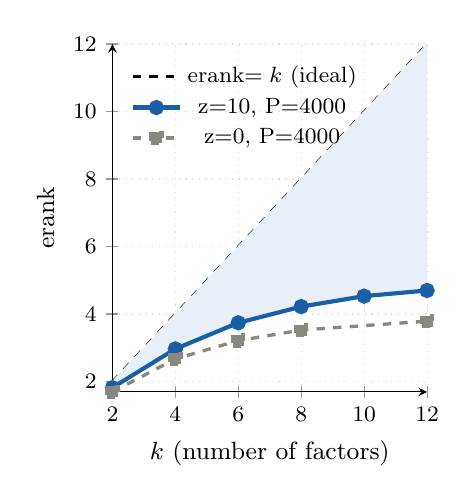
\begin{tikzpicture}
\begin{axis}[
  xlabel={$k$ (number of factors)},
  ylabel={erank},
  xtick={2,4,6,8,10,12},
  legend pos=north west,
  title style={font=\small},
]
% erank = k diagonal
\addplot[black, dashed, thick, domain=2:12, samples=50] {x};
\addlegendentry{erank$=k$ (ideal)}

% fill between diagonal and z=10
\addplot[cblue!10, fill, forget plot]
  coordinates {(2,2)(4,4)(6,6)(8,8)(10,10)(12,12)
               (12,4.697514)(10,4.530078)(8,4.219013)(6,3.740098)(4,2.965567)(2,1.819185)} -- cycle;

% z=10 (Run 3)
\addplot[cblue, mark=*, mark size=2pt, line width=1.5pt]
  coordinates {(2,1.819185)(4,2.965567)(6,3.740098)(8,4.219013)(10,4.530078)(12,4.697514)};
\addlegendentry{z=10, P=4000}

% z=0 (Run 6, k=2,4,6,8,12)
\addplot[cgray, dashed, mark=square*, mark size=2pt, line width=1.2pt]
  coordinates {(2,1.691659)(4,2.669510)(6,3.213275)(8,3.524702)(12,3.788623)};
\addlegendentry{z=0, P=4000}

\end{axis}
\end{tikzpicture}
\caption{erank (solid/dashed) vs the erank$=k$ diagonal (black dashed). Shaded area =
noise contamination predicted by Theorem~6.1(iii). Gap widens with $k$;
steepening near $k=8$--$12$ marks $k_0$.}
\end{figure}

\subsection*{erank peaks at $P\approx 1000$--$4000$ — parameter vs structural complexity}

At fixed $k=4$, $z=10$, erank rises from 3.04 at $P=64$ to a peak near $P=256$--$1000$,
then declines to 2.90 at $P=12{,}000$. This non-monotone behaviour maps to Section~3.5:
RFF lifting enlarges the admissible subspace family (parameter complexity) but
additional flexibility is structurally meaningful only if it yields persistent
increases in intrinsic dimension. Beyond $P\approx 1000$ the RFF approximation
introduces more noise directions than signal, and erank declines.
The spectral gap does not show this P-dependence — confirming the paper's
separation between parameter and structural complexity.

\begin{figure}[h]
\centering
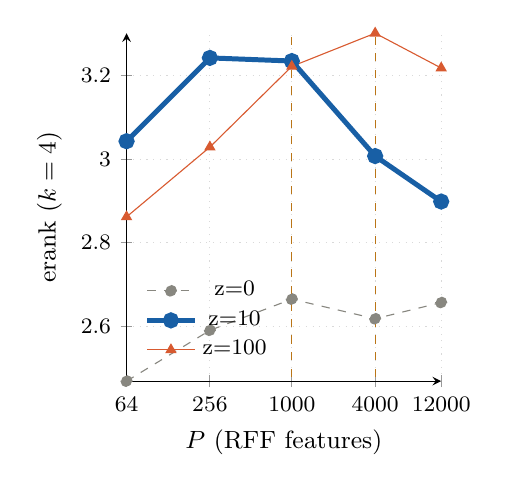
\begin{tikzpicture}
\begin{semilogxaxis}[
  xlabel={$P$ (RFF features)},
  ylabel={erank ($k=4$)},
  xtick={64,256,1000,4000,12000},
  xticklabels={64,256,1000,4000,12000},
  legend pos=south west,
]
% z=0
\addplot[cgray, dashed, mark=*, mark size=2pt]
  coordinates {(64,2.469392)(256,2.590714)(1000,2.665316)(4000,2.618443)(12000,2.657147)};
\addlegendentry{z=0}

% z=10
\addplot[cblue, mark=*, mark size=2pt, line width=1.8pt]
  coordinates {(64,3.042618)(256,3.241705)(1000,3.234208)(4000,3.007169)(12000,2.898490)};
\addlegendentry{z=10}

% z=100
\addplot[ccoral, mark=triangle*, mark size=2pt]
  coordinates {(64,2.861843)(256,3.028680)(1000,3.221386)(4000,3.300722)(12000,3.217489)};
\addlegendentry{z=100}

% peak zone annotation
\draw[camber, dashed, thin] (axis cs:1000,2.4) -- (axis cs:1000,3.35);
\draw[camber, dashed, thin] (axis cs:4000,2.4) -- (axis cs:4000,3.35);
\node[font=\tiny, color=camber] at (axis cs:2000,2.45) {peak zone};

\end{semilogxaxis}
\end{tikzpicture}
\caption{erank vs $P$ at $k=4$ for three regularisation values.
The non-monotone shape: erank peaks then declines beyond $P\approx 1000$--$4000$.
The spectral gap does not show this behaviour, confirming the Section~3.5
parameter/structural complexity separation.}
\end{figure}

\noindent\rule{\textwidth}{0.4pt}

% ═══════════════════════════════════════════════════════════
\section*{Finding 2 — Spectral gap: the strongest diagnostic}

\begin{anngreen}
\small\textbf{Geometry of Complexity — Theorem~6.1(ii) and 6.1(iii).}
Theorem~6.1(iii): $\mathrm{spec}(\Sigma^*_f)=\{\lambda_1,\ldots,\lambda_{k_0},\sigma^2,\ldots,\sigma^2\}$.
The spectral gap $\mathrm{sg}=\lambda_k/\lambda_1$ collapses toward $\sigma^2/\lambda_1$ as
$k$ exceeds $k_0$. Theorem~6.1(ii): $\mathrm{Hess}J \propto \sum(\lambda_i-\sigma^2)\|\xi_i\|^2$;
regularisation raises eigenvalue gaps, increasing curvature.
\end{anngreen}

In the joint $(k,z)$ grid (Run~6, 30 configurations), the spectral gap is
monotonically decreasing in $k$ and monotonically increasing in $z$ — no exceptions.
The key structural feature is the \textbf{98\% relative collapse from $k=8$ to $k=12$},
present at every $z$ value (96--99\%). All earlier steps show 60--77\% drops.
This structural break is independent of regularisation, identifying $k_0\approx 8$.
At $k=12$ the gap is essentially zero at every $z$ (0.0001--0.0005).
Critically, the spectral gap is P-independent (CV$<7\%$ across all $P$ values).

\begin{figure}[h]
\centering
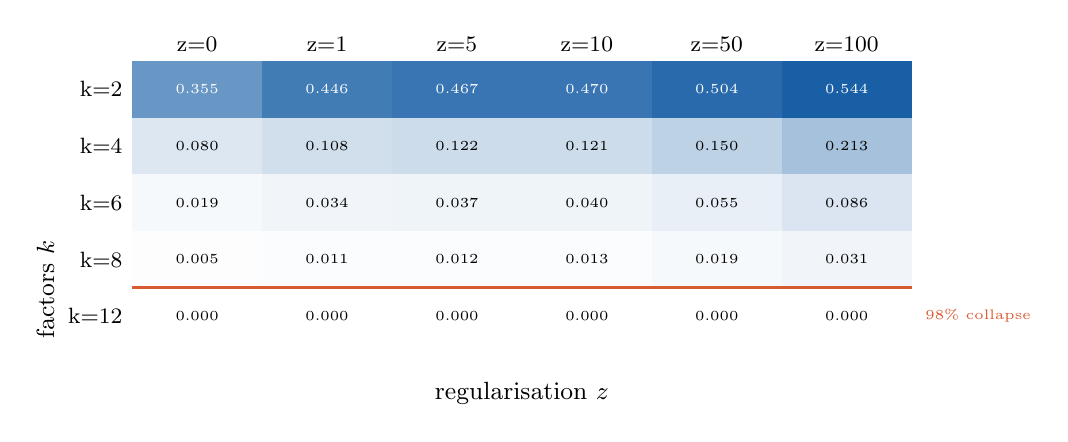
\begin{tikzpicture}[font=\footnotesize]
  \fill[cblue!65!white] (0.000,0.000) rectangle (1.650,0.720);
  \node[white, font=\tiny] at (0.825,0.360) {0.355};
  \fill[cblue!82!white] (1.650,0.000) rectangle (3.300,0.720);
  \node[white, font=\tiny] at (2.475,0.360) {0.446};
  \fill[cblue!86!white] (3.300,0.000) rectangle (4.950,0.720);
  \node[white, font=\tiny] at (4.125,0.360) {0.467};
  \fill[cblue!86!white] (4.950,0.000) rectangle (6.600,0.720);
  \node[white, font=\tiny] at (5.775,0.360) {0.470};
  \fill[cblue!93!white] (6.600,0.000) rectangle (8.250,0.720);
  \node[white, font=\tiny] at (7.425,0.360) {0.504};
  \fill[cblue!100!white] (8.250,0.000) rectangle (9.900,0.720);
  \node[white, font=\tiny] at (9.075,0.360) {0.544};
  \fill[cblue!15!white] (0.000,-0.720) rectangle (1.650,0.000);
  \node[black, font=\tiny] at (0.825,-0.360) {0.080};
  \fill[cblue!20!white] (1.650,-0.720) rectangle (3.300,0.000);
  \node[black, font=\tiny] at (2.475,-0.360) {0.108};
  \fill[cblue!22!white] (3.300,-0.720) rectangle (4.950,0.000);
  \node[black, font=\tiny] at (4.125,-0.360) {0.122};
  \fill[cblue!22!white] (4.950,-0.720) rectangle (6.600,0.000);
  \node[black, font=\tiny] at (5.775,-0.360) {0.121};
  \fill[cblue!28!white] (6.600,-0.720) rectangle (8.250,0.000);
  \node[black, font=\tiny] at (7.425,-0.360) {0.150};
  \fill[cblue!39!white] (8.250,-0.720) rectangle (9.900,0.000);
  \node[black, font=\tiny] at (9.075,-0.360) {0.213};
  \fill[cblue!4!white] (0.000,-1.440) rectangle (1.650,-0.720);
  \node[black, font=\tiny] at (0.825,-1.080) {0.019};
  \fill[cblue!6!white] (1.650,-1.440) rectangle (3.300,-0.720);
  \node[black, font=\tiny] at (2.475,-1.080) {0.034};
  \fill[cblue!7!white] (3.300,-1.440) rectangle (4.950,-0.720);
  \node[black, font=\tiny] at (4.125,-1.080) {0.037};
  \fill[cblue!7!white] (4.950,-1.440) rectangle (6.600,-0.720);
  \node[black, font=\tiny] at (5.775,-1.080) {0.040};
  \fill[cblue!10!white] (6.600,-1.440) rectangle (8.250,-0.720);
  \node[black, font=\tiny] at (7.425,-1.080) {0.055};
  \fill[cblue!16!white] (8.250,-1.440) rectangle (9.900,-0.720);
  \node[black, font=\tiny] at (9.075,-1.080) {0.086};
  \fill[cblue!1!white] (0.000,-2.160) rectangle (1.650,-1.440);
  \node[black, font=\tiny] at (0.825,-1.800) {0.005};
  \fill[cblue!2!white] (1.650,-2.160) rectangle (3.300,-1.440);
  \node[black, font=\tiny] at (2.475,-1.800) {0.011};
  \fill[cblue!2!white] (3.300,-2.160) rectangle (4.950,-1.440);
  \node[black, font=\tiny] at (4.125,-1.800) {0.012};
  \fill[cblue!2!white] (4.950,-2.160) rectangle (6.600,-1.440);
  \node[black, font=\tiny] at (5.775,-1.800) {0.013};
  \fill[cblue!4!white] (6.600,-2.160) rectangle (8.250,-1.440);
  \node[black, font=\tiny] at (7.425,-1.800) {0.019};
  \fill[cblue!6!white] (8.250,-2.160) rectangle (9.900,-1.440);
  \node[black, font=\tiny] at (9.075,-1.800) {0.031};
  \fill[cblue!0!white] (0.000,-2.880) rectangle (1.650,-2.160);
  \node[black, font=\tiny] at (0.825,-2.520) {0.000};
  \fill[cblue!0!white] (1.650,-2.880) rectangle (3.300,-2.160);
  \node[black, font=\tiny] at (2.475,-2.520) {0.000};
  \fill[cblue!0!white] (3.300,-2.880) rectangle (4.950,-2.160);
  \node[black, font=\tiny] at (4.125,-2.520) {0.000};
  \fill[cblue!0!white] (4.950,-2.880) rectangle (6.600,-2.160);
  \node[black, font=\tiny] at (5.775,-2.520) {0.000};
  \fill[cblue!0!white] (6.600,-2.880) rectangle (8.250,-2.160);
  \node[black, font=\tiny] at (7.425,-2.520) {0.000};
  \fill[cblue!0!white] (8.250,-2.880) rectangle (9.900,-2.160);
  \node[black, font=\tiny] at (9.075,-2.520) {0.000};
  \node[left, font=\footnotesize] at (0, 0.360) {k=2};
  \node[left, font=\footnotesize] at (0, -0.360) {k=4};
  \node[left, font=\footnotesize] at (0, -1.080) {k=6};
  \node[left, font=\footnotesize] at (0, -1.800) {k=8};
  \node[left, font=\footnotesize] at (0, -2.520) {k=12};
  \node[above, font=\footnotesize] at (0.825, 0.720) {z=0};
  \node[above, font=\footnotesize] at (2.475, 0.720) {z=1};
  \node[above, font=\footnotesize] at (4.125, 0.720) {z=5};
  \node[above, font=\footnotesize] at (5.775, 0.720) {z=10};
  \node[above, font=\footnotesize] at (7.425, 0.720) {z=50};
  \node[above, font=\footnotesize] at (9.075, 0.720) {z=100};
  \node[below, font=\small] at (4.950, -3.24) {regularisation $z$};
  \node[left, font=\small, rotate=90] at (-1.1, -1.44) {factors $k$};
  \draw[ccoral, very thick] (0, -2.16) -- (9.90, -2.16);
  \node[ccoral, right, font=\tiny] at (9.95, -2.52) {98\% collapse};
\end{tikzpicture}
\caption{Spectral gap ratio heatmap. Monotone in both dimensions without exception.
Coral line marks the $k=8\to12$ boundary where 98\% structural collapse occurs
at every $z$. The $k=12$ row is near-zero for all $z$.}
\end{figure}

\noindent\rule{\textwidth}{0.4pt}

% ═══════════════════════════════════════════════════════════
\section*{Finding 3 — Sharpe: virtuous arc only visible with regularisation}

{\small\color{cgray}
With only 60 monthly portfolio return observations, the standard error on an
annualised Sharpe of $\approx 0.5$ is approximately 0.13.
Differences smaller than this are statistically indistinguishable.
Read these plots for qualitative pattern rather than precise values.}

\medskip
At $z=0$ (illusory regime) Sharpe is flat and low across all $k$ — no $k$ selection
helps. At $z=10$ a clear arc emerges, peaking at $k=8$ (Sharpe$=0.591$) and
declining at $k=12$. At $z=100$ a similar but lower arc appears. This maps to
Section~7: complexity is virtuous if out-of-sample performance improves with $k$.
Here it only improves when the model is in the virtuous regime ($z\geq 10$).
The peak at $k=8$ corroborates $k_0\approx 8$ identified from the spectral gap.

The scatter plot below shows Sharpe against the spectral gap for all 30 $(k,z)$ cells.
Within each $k$, higher spectral gap does not reliably predict higher Sharpe.
This is consistent with the paper: the spectral gap diagnoses factor identification
quality (Section~7 criterion ii--iii) while Sharpe diagnoses performance (criterion iv).
Both are necessary; they are complementary, not redundant.

\begin{figure}[h]
\centering
\begin{subfigure}[b]{0.48\textwidth}
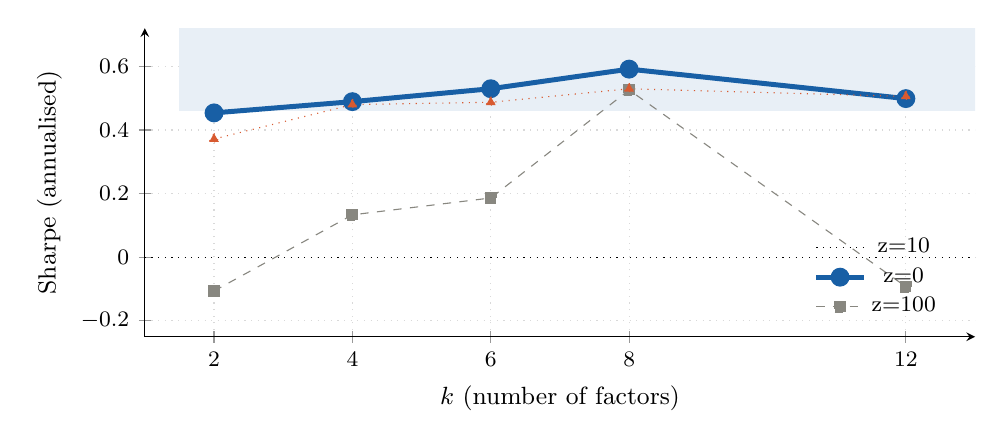
\begin{tikzpicture}
\begin{axis}[
  xlabel={$k$ (number of factors)},
  ylabel={Sharpe (annualised)},
  xtick={2,4,6,8,12},
  ymin=-0.25, ymax=0.72,
  legend pos=south east,
  height=5.5cm,
  width=\textwidth,
]
% zero line
\addplot[black, dotted, domain=1:13] {0};

% ±1 SE band around k=8 z=10 peak
\addplot[cblue!10, fill between/.style={}, forget plot, fill=cblue!10]
  coordinates {(1.5,0.461)(13,0.461)(13,0.721)(1.5,0.721)};

% z=10
\addplot[cblue, mark=*, mark size=2.5pt, line width=1.8pt]
  coordinates {(2,0.453775)(4,0.489134)(6,0.529764)(8,0.591410)(12,0.498729)};
\addlegendentry{z=10}

% z=0
\addplot[cgray, dashed, mark=square*, mark size=2pt]
  coordinates {(2,-0.106219)(4,0.133285)(6,0.186250)(8,0.525911)(12,-0.092654)};
\addlegendentry{z=0}

% z=100
\addplot[ccoral, dotted, mark=triangle*, mark size=2pt]
  coordinates {(2,0.371712)(4,0.479894)(6,0.487193)(8,0.529622)(12,0.505495)};
\addlegendentry{z=100}

\end{axis}
\end{tikzpicture}
\caption{Sharpe vs $k$. Shaded band = $\pm1$ SE at $k=8$.
Only $z=10$ shows a virtuous arc.}
\end{subfigure}
\hfill
\begin{subfigure}[b]{0.48\textwidth}
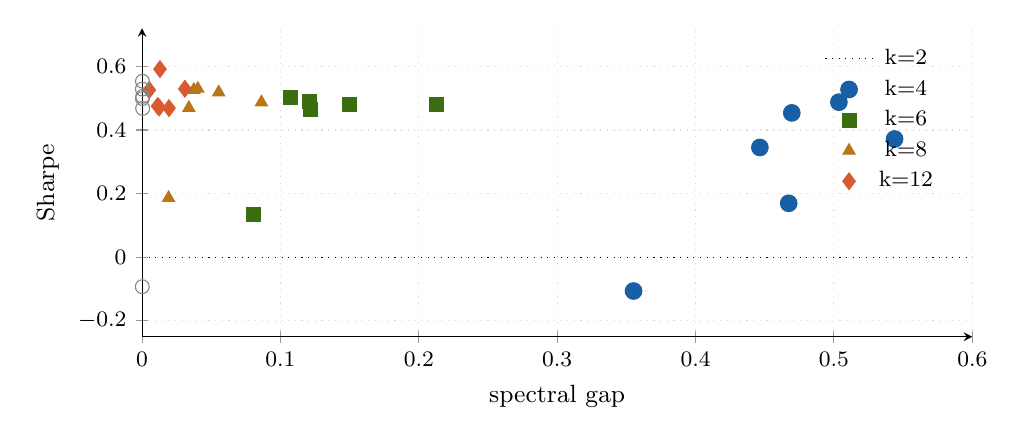
\begin{tikzpicture}
\begin{axis}[
  xlabel={spectral gap},
  ylabel={Sharpe},
  ymin=-0.25, ymax=0.72,
  legend pos=north east,
  height=5.5cm,
  width=\textwidth,
]
\addplot[black, dotted, domain=0:0.6] {0};

% k=2
\addplot[cblue, only marks, mark=*, mark size=3pt]
  coordinates {(0.355187,-0.106219)(0.446481,0.345069)(0.467332,0.169554)
               (0.469553,0.453775)(0.503588,0.487521)(0.543827,0.371712)};
\addlegendentry{k=2}

% k=4
\addplot[cgreen, only marks, mark=square*, mark size=2.5pt]
  coordinates {(0.080208,0.133285)(0.107582,0.501508)(0.121900,0.465083)
               (0.121232,0.489134)(0.150029,0.478797)(0.212784,0.479894)};
\addlegendentry{k=4}

% k=6
\addplot[camber, only marks, mark=triangle*, mark size=2.5pt]
  coordinates {(0.019166,0.186250)(0.033816,0.469259)(0.037400,0.526327)
               (0.040315,0.529764)(0.055366,0.518383)(0.086269,0.487193)};
\addlegendentry{k=6}

% k=8
\addplot[ccoral, only marks, mark=diamond*, mark size=3pt]
  coordinates {(0.005185,0.525911)(0.011262,0.475151)(0.012409,0.471003)
               (0.012937,0.591410)(0.019451,0.468764)(0.030926,0.529622)};
\addlegendentry{k=8}

% k=12
\addplot[cgray, only marks, mark=o, mark size=2.5pt]
  coordinates {(0.000127,-0.092654)(0.000420,0.467994)(0.000269,0.553379)
               (0.000262,0.498729)(0.000235,0.528739)(0.000459,0.505495)};
\addlegendentry{k=12}

\end{axis}
\end{tikzpicture}
\caption{Sharpe vs spectral gap. No systematic within-$k$ relationship:
diagnostics and performance are complementary.}
\end{subfigure}
\caption{Sharpe plots (Run~6, $P=4000$). Left: virtuous arc appears only at $z\geq10$.
Right: spectral gap predicts factor structure quality, not performance directly.}
\end{figure}

\noindent\rule{\textwidth}{0.4pt}

% ═══════════════════════════════════════════════════════════
\section*{Summary mapping}

\renewcommand{\arraystretch}{1.25}
\begin{tabular}{>{\bfseries\small}p{3.2cm} p{3.8cm} p{4.0cm} p{2.6cm}}
\rowcolor{headbg}\color{headfg} Finding &
\color{headfg} Theorem / Section &
\color{headfg} Evidence &
\color{headfg} Strength \\
\hline
erank gap from diagonal grows with $k$ &
Thm~6.1(iii) block spectral structure &
Gap tracks $k-k_0$ noise dims &
\textcolor{cblue}{Strong} \\
\rowcolor{rowalt}
erank peaks at $P\sim1000$--$4000$ &
Section~3.5 param vs structural &
Non-monotone in $P$ at every $z$ &
\textcolor{camber}{Moderate} \\
Spectral gap 98\% collapse at $k=8{\to}12$ &
Thm~6.1(iii) block spectral structure &
98\% drop at all 6 $z$ values, P-independent &
\textcolor{cblue}{Strong --- $k_0\approx8$} \\
\rowcolor{rowalt}
Spectral gap monotone in $k$ and $z$ &
Thm~6.1(ii)+(iii) &
30/30 cells, no exceptions &
\textcolor{cblue}{Strong} \\
Sharpe arc at $z=10$, flat at $z=0$ &
Section~7 virtuous vs illusory &
Peak 0.591 at $k=8$; SE$\approx0.13$ &
\textcolor{camber}{Moderate, directional} \\
\rowcolor{rowalt}
$d_{\mathrm{proj}}$ saturates at $\sqrt{2k}$ &
Cannot confirm Thm~6.1(i) &
Matches Haar-random formula to 0.01\% &
\textcolor{cred}{Unreliable: warm-start needed} \\
\end{tabular}

\noindent\rule{\textwidth}{0.4pt}

% ═══════════════════════════════════════════════════════════
\section*{Finding 4 — $d_{\mathrm{proj}}$ is unreliable: random restarts explain the saturation}

\begin{annred}
\small\textbf{Why $d_{\mathrm{proj}}$ cannot confirm Theorem~6.1(i) in the current setup.}
Theorem~6.1(i) predicts flat Hessian directions produce $O(1)$ subspace rotations.
However, the backtest uses a fresh random $W_0$ at every rolling window.
Two points drawn from the Haar-uniform measure on $\mathrm{Gr}(m,k)$ have
$\mathbb{E}[d_{\mathrm{proj}}^2] = 2k(m-k)/(m+1)$, which approaches $2k$ as $m=P$ grows
--- regardless of loss curvature. The flat Hessian and random restarts produce identical
$d_{\mathrm{proj}}$ signatures and cannot be distinguished without warm-starting.
\end{annred}

At $m=P=4000$, $k=6$: the Haar formula gives $\mathbb{E}[d_{\mathrm{proj}}]=3.461$
and we observe $3.461$. The ratio observed/expected$_{\mathrm{random}}=1.0001$.
This holds at every $(k,P,z=0)$ configuration tested.
One partial observation survives: at small $P=64$, $z=10$ gives $d_{\mathrm{proj}}=1.51$
(53\% of max) vs $z=0$ at 1.95 (98\% of max), a genuine gap since the Haar baseline
at $P=64$ is only 97.7\% of max.
\textbf{The fix is one line:} pass \texttt{initial\_point=W\_prev} to \texttt{est.fit()}.

\begin{figure}[h]
\centering
\begin{subfigure}[b]{0.48\textwidth}
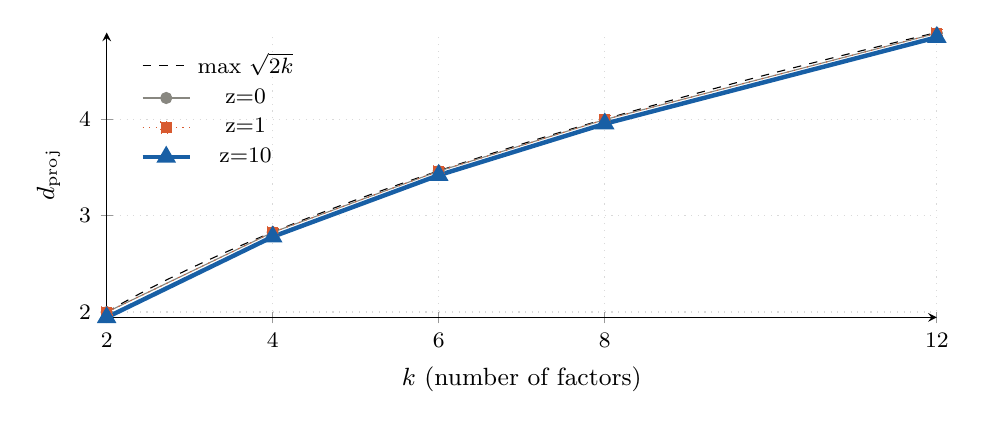
\begin{tikzpicture}
\begin{axis}[
  xlabel={$k$ (number of factors)},
  ylabel={$d_{\mathrm{proj}}$},
  xtick={2,4,6,8,12},
  legend pos=north west,
  height=5.2cm, width=\textwidth,
]
% max sqrt(2k) curve
\addplot[black, dashed, domain=2:12, samples=60] {sqrt(2*x)};
\addlegendentry{max $\sqrt{2k}$}

% z=0
\addplot[cgray, mark=*, mark size=2pt]
  coordinates {(2,1.998565)(4,2.826917)(6,3.461495)(8,3.995945)(12,4.891627)};
\addlegendentry{z=0}

% z=1
\addplot[ccoral, dotted, mark=square*, mark size=2pt]
  coordinates {(2,1.997940)(4,2.826524)(6,3.461186)(8,3.995649)(12,4.891335)};
\addlegendentry{z=1}

% z=10
\addplot[cblue, mark=triangle*, mark size=2.5pt, line width=1.6pt]
  coordinates {(2,1.944254)(4,2.780979)(6,3.419196)(8,3.952290)(12,4.849657)};
\addlegendentry{z=10}

\end{axis}
\end{tikzpicture}
\caption{$d_{\mathrm{proj}}$ vs $k$. All $z$ values near max at $P=4000$;
z=0 and z=1 indistinguishable.}
\end{subfigure}
\hfill
\begin{subfigure}[b]{0.48\textwidth}
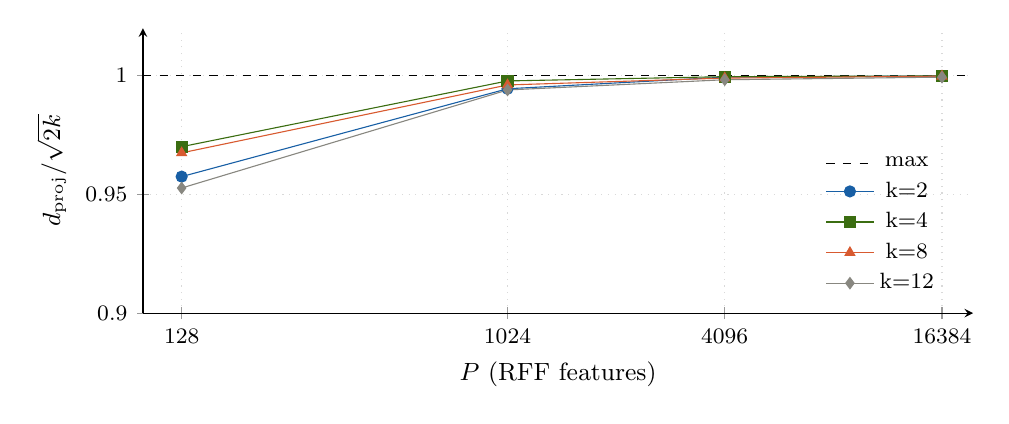
\begin{tikzpicture}
\begin{semilogxaxis}[
  xlabel={$P$ (RFF features)},
  ylabel={$d_{\mathrm{proj}}/\sqrt{2k}$},
  xtick={128,1024,4096,16384},
  xticklabels={128,1024,4096,16384},
  ymin=0.9, ymax=1.02,
  legend pos=south east,
  height=5.2cm, width=\textwidth,
]
\addplot[black, dashed, domain=100:20000] {1.0};
\addlegendentry{max}

% k=2
\addplot[cblue, mark=*, mark size=2pt]
  coordinates {(128,0.9575)(1024,0.9945)(4096,0.9994)(16384,0.9999)};
\addlegendentry{k=2}

% k=4
\addplot[cgreen, mark=square*, mark size=2pt]
  coordinates {(128,0.9701)(1024,0.9978)(4096,0.9996)(16384,0.9999)};
\addlegendentry{k=4}

% k=8
\addplot[ccoral, mark=triangle*, mark size=2pt]
  coordinates {(128,0.9675)(1024,0.9961)(4096,0.9990)(16384,0.9998)};
\addlegendentry{k=8}

% k=12
\addplot[cgray, mark=diamond*, mark size=2pt]
  coordinates {(128,0.9527)(1024,0.9940)(4096,0.9983)(16384,0.9994)};
\addlegendentry{k=12}

\end{semilogxaxis}
\end{tikzpicture}
\caption{$d_{\mathrm{proj}}/\sqrt{2k}$ vs $P$ at $z=0$. All $k$ converge to 1.0
as $P$ grows — matching the Haar-random expectation.}
\end{subfigure}
\caption{$d_{\mathrm{proj}}$ plots (Run~6 left, Run~2 right). Saturation is driven by
ambient Grassmannian geometry, not loss curvature.}
\end{figure}

% ═══════════════════════════════════════════════════════════
\section*{Open questions and caveats}

\textbf{Warm-start — critical fix required.}
The fix is one line in the rolling loop: \texttt{initial\_point=W\_prev}.
Until done, all $d_{\mathrm{proj}}$-based conclusions are provisional.

\medskip
\textbf{Kelly mapping incomplete.}
Both Kelly papers (2024 \emph{Journal of Finance}; 2025 SSRN) are cited by the
Geometry of Complexity paper but could not be read directly.
The Sharpe-based complexity scaling test requires $N\gg 35$ to have statistical power.

\medskip
\textbf{$k_0$ is estimated, not formally identified.}
The spectral gap 98\% collapse at $k=8\to12$ and Sharpe peak at $k=8$
suggest $k_0\approx 8$ for this 35-stock universe.
A formal test using Theorem~5.1 (fitting at $k=k_0$ should yield a unique minimiser)
has not been implemented.

\end{document}
